\documentclass{article}
\usepackage{enumitem}
\usepackage{listings}
\usepackage{amsfonts}
\usepackage{latexsym}
\usepackage{fullpage}
\usepackage{graphicx}
\usepackage{paralist}
\usepackage{tikz-timing}

\lstdefinelanguage{VHDL}{
  morekeywords={
    library,use,all,ENTITY,IS,PORT,IN,OUT,end,architecture,of,
    begin,and, ARCHITECTURE, IF, THEN, SIGNAL,END, PROCESS
  },
  morecomment=[l]--
}

\usepackage{xcolor}
\colorlet{keyword}{blue!100!black!80}
\colorlet{comment}{green!90!black!90}
\lstdefinestyle{vhdl}{
  language     = VHDL,
  basicstyle   = \ttfamily\scriptsize,
  keywordstyle = \color{keyword}\bfseries\ttfamily,
  commentstyle = \color{comment}\ttfamily,	
  tabsize=1
}

\renewcommand{\lstlistingname}{Code}

% Default margins are too wide all the way around. I reset them here
\setlength{\topmargin}{-.5in}
\setlength{\textheight}{9in}
\setlength{\oddsidemargin}{.125in}
\setlength{\textwidth}{6.25in}


%\let\oldenumerate\enumerate
%\renewcommand{\enumerate}{
  %\oldenumerate
  %\setlength{\itemsep}{1pt}
  %\setlength{\parskip}{0pt}
  %\setlength{\parsep}{0pt}
%}


\begin{document}
\title{EECS112L Organization of Digital Computers Lab}
\author{\textbf{Final Project} \textbf{Pipeline ARM} \\ \\
Group name: Three Musketeers \\ \\ Group ID: 118 \\ \\ Student name: \\ Raymond Wang \\ Jared Lim\\ Heyang Chen \\ \\ Student ID: \\17769107~\\31633414~\\55554499~\\ \\ 
EECS Department\\ Henry Samueli School of Engineering \\ University of California, Irvine \\ \\
{March, 24, 2017}} 


\date{}
\maketitle

\newpage

\section{Description of this Lab}

In this lab, We implemented a five stage pipeline processor according to the single cycle ARM processor we designed in last lab.

\section{Block Diagram}

This is the block diagram of the single cycle processor from last time.
\newline
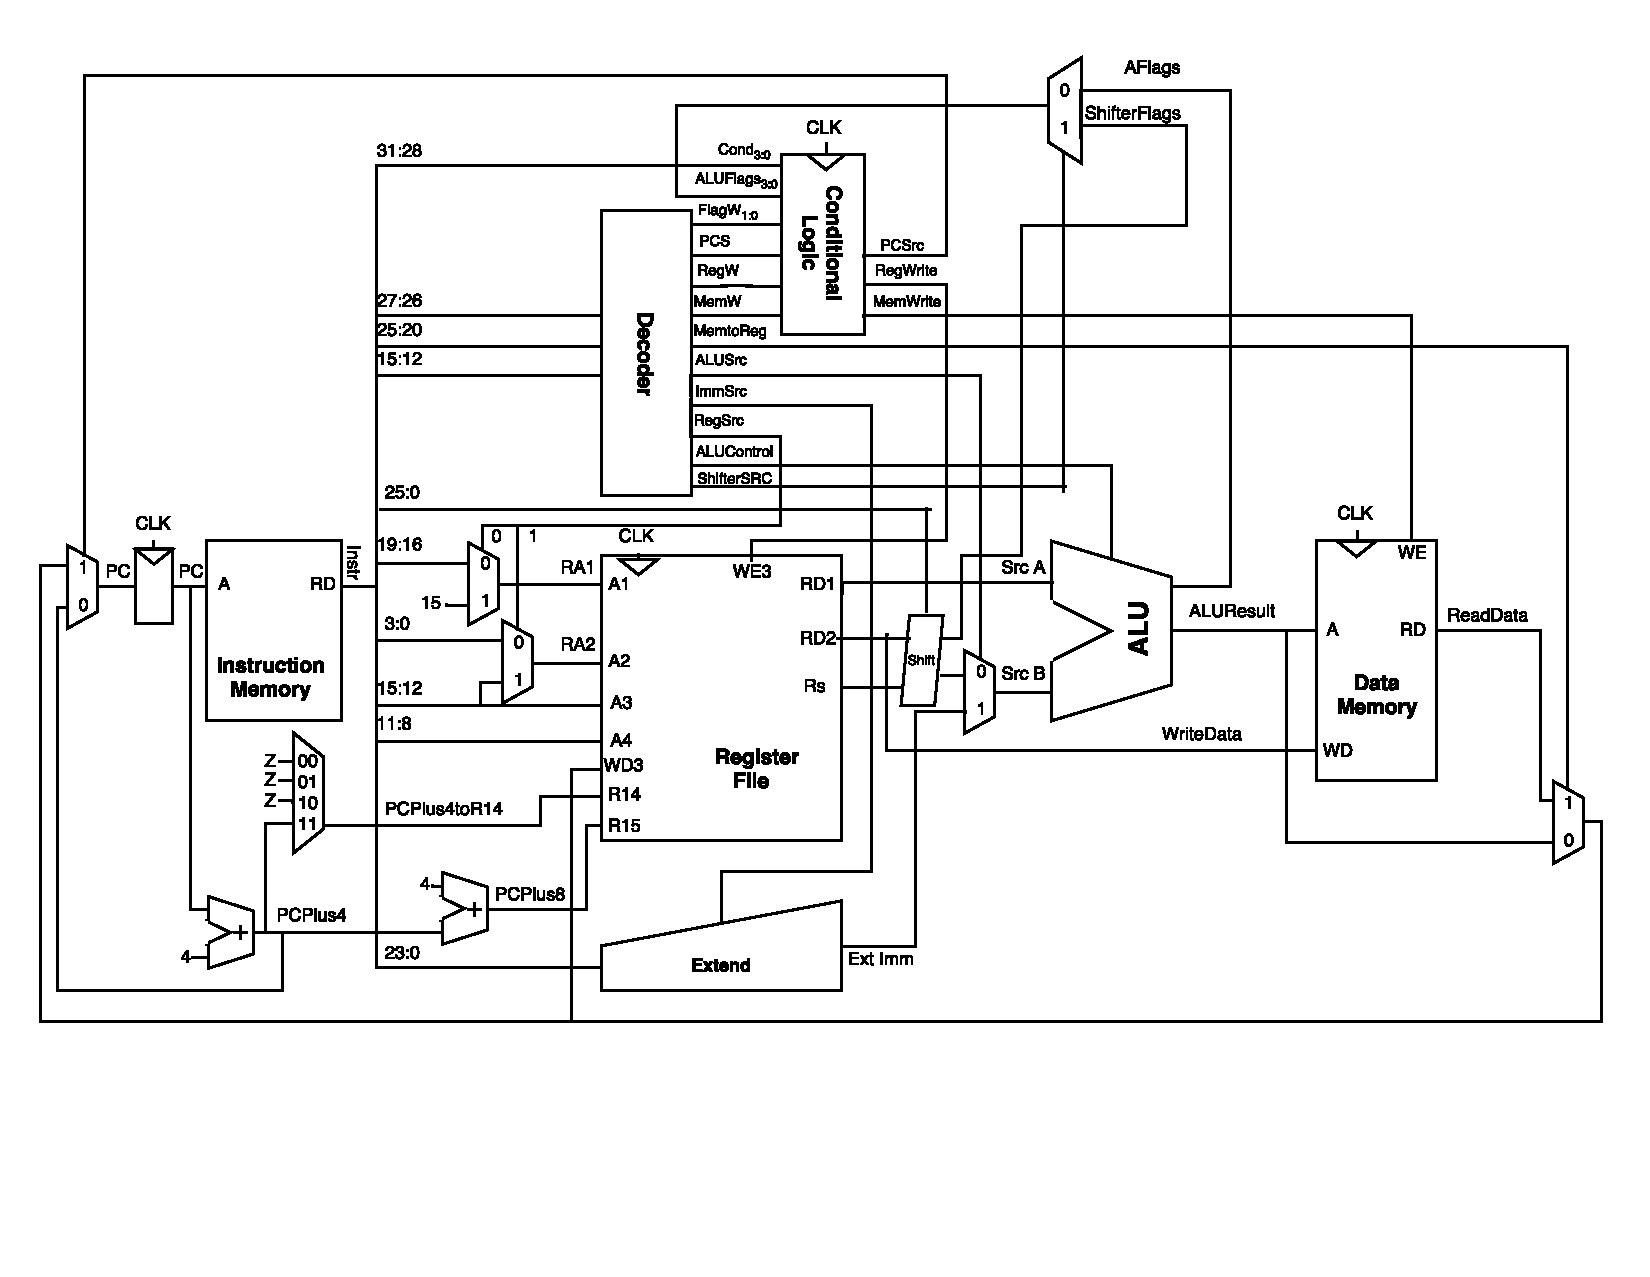
\includegraphics[width=1.0\textwidth]{SingleCycleProcessor.pdf}
\newline
This is the block diagram of pipeline processor with control.
\newline
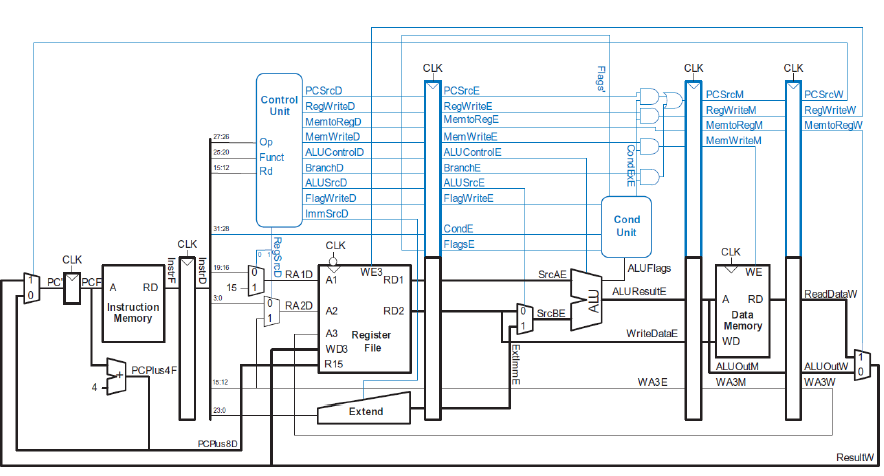
\includegraphics[width=1.0\textwidth]{Blockdiagramwithpp.png}
\newline
This is the block diagram that able to handle hazard control including forwarding and stalling.
\newline
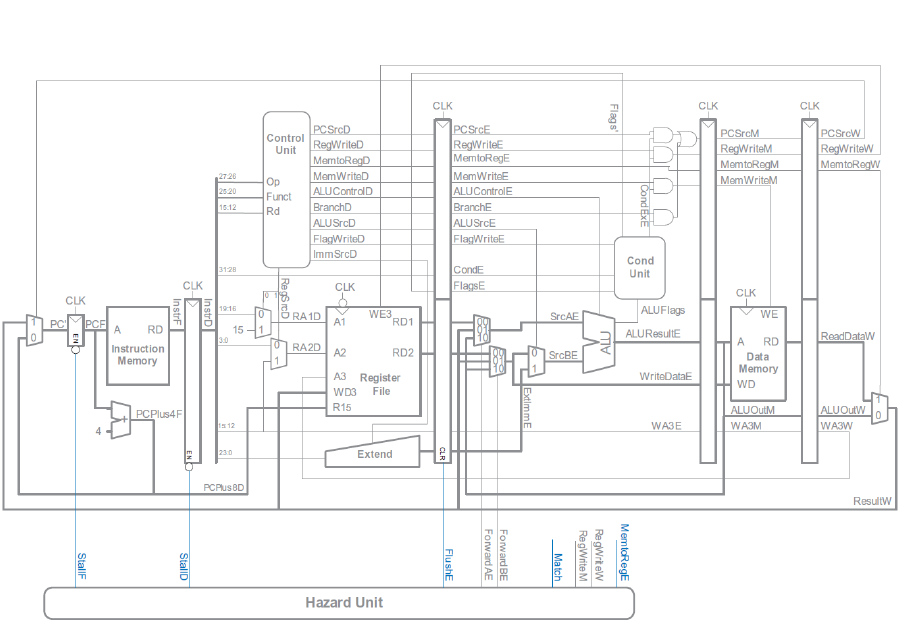
\includegraphics[width=1.0\textwidth]{Blockdiagramwithhu.png}
\newline
These block diagrams for pipeline processor did not include features like shifter or PCPlus4toR14, but they are actually the same
as the block diagram in single cycle processor. This hand drawn block diagram shows what it should be although it may not be very clear.
\newline
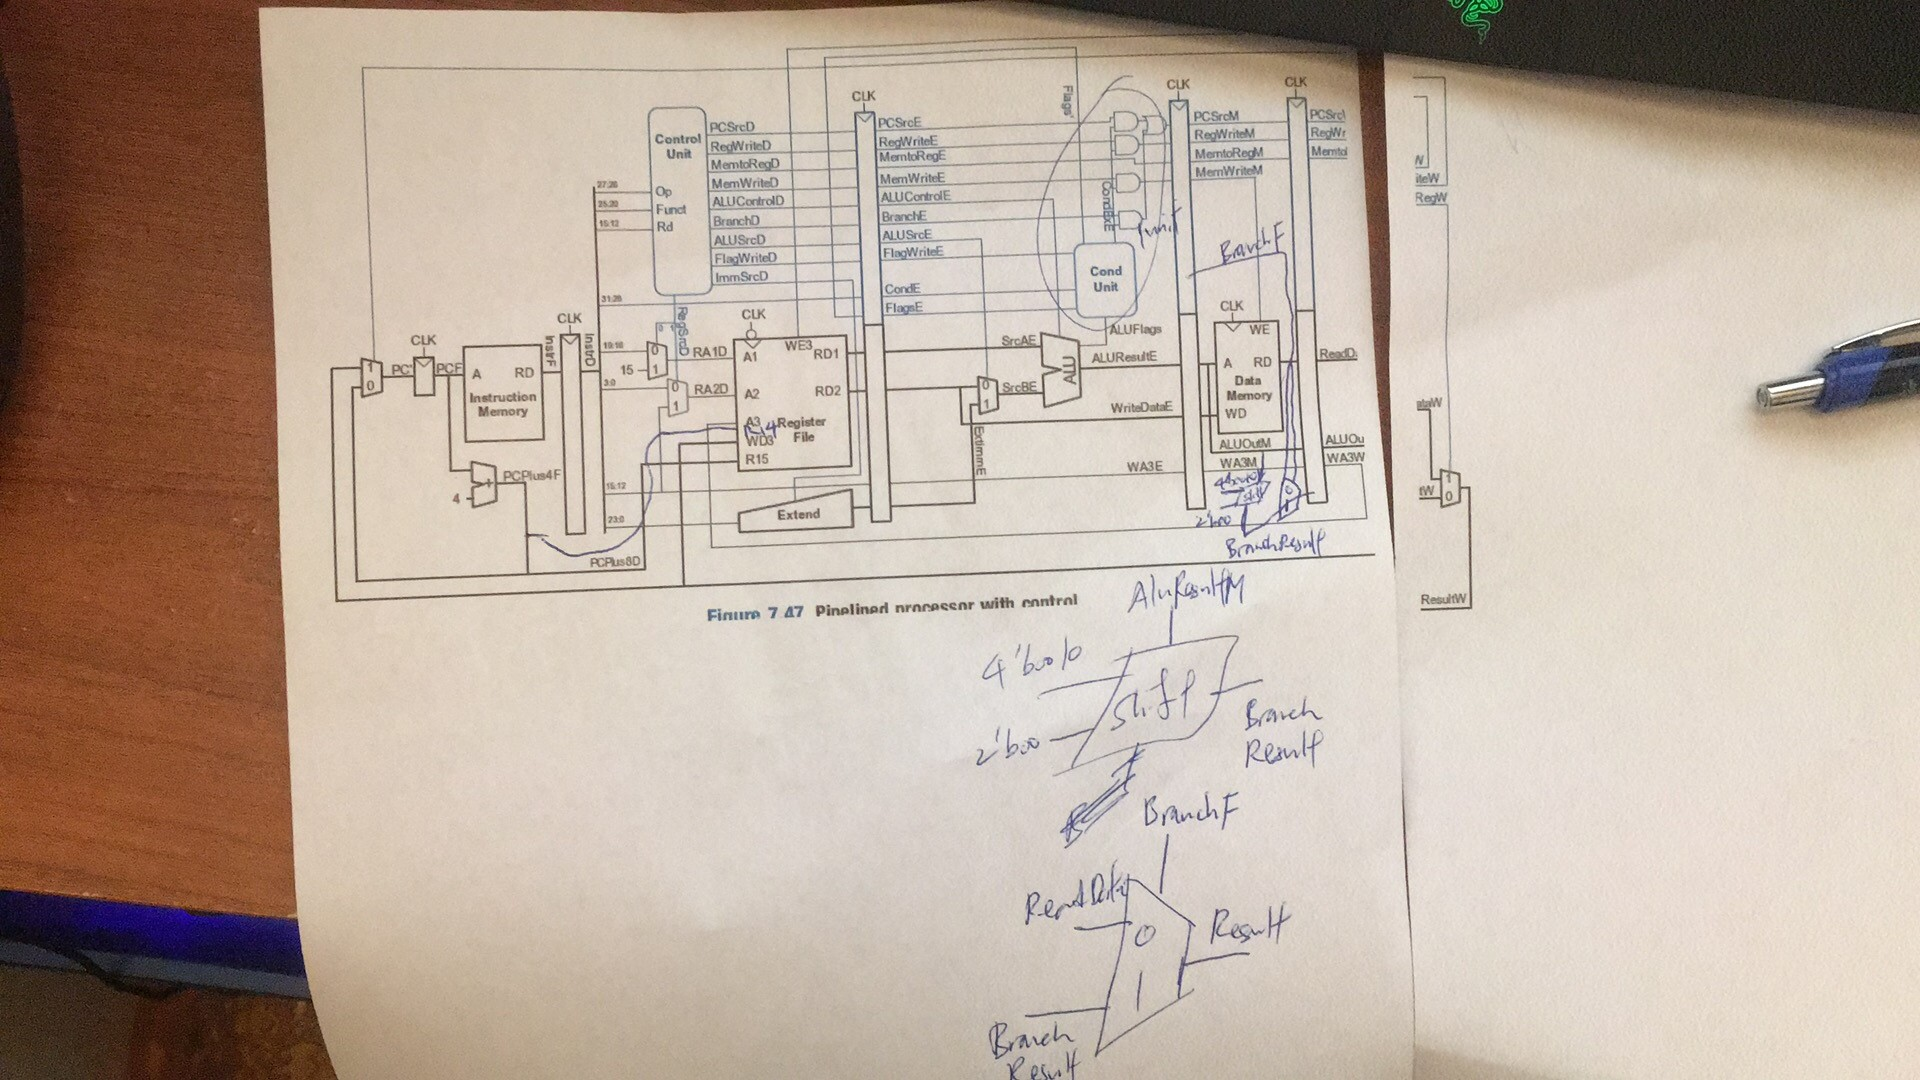
\includegraphics[width=1.0\textwidth]{hdbd.jpg}

\section{Design Architecture}

For the design of five stage pipeline processor, it is separated in three steps as indicated in project description.
\newline
First of all, we have designed four pipeline registers, which separate a single cycle processor into five stages, Fetch, Decode, Execute, Memory, and Writeback. These pipeline registers takes not only logics coming out from modules such as regfile, ALU but also takes control signals. Also in this step, we have the conditional logic separated from its formal place control unit but put it individually in execute  stage as conditional unit.
\newline
In the second stage, we design a hazard unit, which takes signal regwrite at both memory stage and writeback stage, and also 4 matching signals. Then it output ForwardAE and ForwardBE, which are signals to use in two 4 way multiplexer to decide whether the result can be directly forward back to use as SrcA or SrcB.
\newline
At last, we edited hazard unit by adding one more matching signal input, and memtoreg signal at execute stage into it, while also having it output StallF, StallD and FlushE. When these signals are received in pipeline register, the pipeline register will stall the current situation and add NOP into it. When stall ends, the pipeline register will work again.

\section{Simulation Waveform}




\end{document}
